
%-----------------------------------------------------------------------------
\chapter{Epistatic GWAS analysis\label{ch:gwas}}
%-----------------------------------------------------------------------------

%---
\section{Preface}
%---


In recent years, over 80 genetic loci related to T2D have been identified \cite{morris2012large, consortium2014genome}. Nevertheless, the overall effect sizes of these loci account for less than 10\% of the overall disease predisposition \cite{manolio2009finding}. This poses the question of why, given that so much efforts has been directed at finding the genetic components of this disease, the loci found so far have such modest effects. This lack of large genetic effects, known as the ``missing heritability" problem, does not only arise in T2D but also in almost all complex traits. In recent studies about missing heritability \cite{zuk2012mystery, zuk2014searching} it was proposed that this effect might be partly explained by taking into account epistasis (i.e. gene interactions).

In this chapter, we propose a novel framework that takes into account putative epistatic interactions into genome wide association studies (GWAS). 

%We detect putative interactions by means of a co-evolutionary model that we develop based on Markov evolutionary theory. We fit the co-evolutionary model's parameters using protein structural data (PDB) an genome wide multiple sequence alignments (UCSC's 100-way). Once this model is parametrized, we perform genome wide association using of pairs of variants  from a sequencing study by incorporating the co-evolutionary model as priors in a Bayesian Framework.

Although this thesis focusses on the development of computational approaches that could be applied to the study of a number of complex diseases, our focus has been on type II diabetes mellitus (T2D), a complex disease first described by the Egyptians in 1500 BCE. Later the Greeks in 230 BCE used the term ``diabetes" meaning ``pass through" (or ``siphon") denoting the constant thirst and frequent urination of the patients. In the 1700s the term ``mellitus" (from honey) was added to denote that the urine was sweet and would ``attracts ants".

Diabetes symptoms include frequent urination, thirst, and constant hunger, high blood sugar (hyperglycemia) and insulin resistance. Long term complication from T2D may include eyesight problems, heart disease, strokes and kidney failure. Type II diabetes, is highly correlated with obesity and disease rate has increased dramatically during the last 50 years. According to the World Health Organisation the prevalence of diabetes is 9\% in adults and an estimated 1.5 millions deaths were caused by diabetes in 2012 \cite{guariguata2014global}, which is predicted to be the 7th leading cause of death by 2030. The costs associated to treating diabetes patients only in the U.S. are estimated around \$245 billion dollars.

The rest of the chapter is published in: \textbf{P. Cingolani}, R. Sladek, M. Blanchette, ``A co-evolutionary approach for detecting epistatic interactions in genome-wide association studies"

%---
\section{Abstract}
%---

\paragraph{Motivation} Epistasis, broadly defined as genetic interactions, is one of the likely causes why genome-wide association studies (GWAS) account for a small portion of heritable disease risk. Due to their high complexity, reduced statistical power and sometimes prohibitive computational requirements, epistatic GWAS have rarely been performed. 

\paragraph{Methods} In this paper, we propose a novel methodology for analysing putative epistatic interactions by combining multiple genome alignments and sequencing information. Using protein structures for individual and co-crystallized complexes information and genome wide multiple species alignment we create a co-evolutionary model that allows the calculation of the posterior probability of physical interaction between residues given evolutionary data. These probabilities are then used as the interaction priors for an epistatic GWAS analysis as basis for genome wide Bayesian framework. 

\paragraph{Results} Our optimized algorithms can be applied to genome wide scale sequencing studies for tens of thousands of samples, that typically yield millions of variants. We applied our approach to a large type II diabetes (T2D) case-control cohort and inferred a number of putative interactions associated with increased risk of developing T2D. 

\paragraph{Availability} Our code is publicly available at \texttt{github.com/pcingola/Epistasis}

%---
\section{Introduction}
%---

Genetic studies aim to discover how a phenotype of interest, such as disease risk or height, is affected by in individual's genetic background. Genome wide association studies (GWAS) are powerful techniques aimed at finding statistical associations between a phenotype and genetic variants \cite{clarke2011basic}. Although several genetic variants related to different phenotypes have been found, variants discovered in GWAS so far can only explain a small part for the phenotypic heritability. For instance, all genetic variants associated to height collectively account for few centimetres in the offspring's height \cite{wood2014defining}. Similarly the known variants related to type 2 diabetes risk collectively explain only 5\% to 10\% of the overall variance in disease predisposition \cite{morris2012large, consortium2014genome}. This problem is known as ``missing heritability" \cite{manolio2009finding} and recent theories suggest that genetic interactions (epistasis) might play an important role in it \cite{zuk2012mystery, zuk2014searching}.

The foundations for epistasis \cite{gao2010classification}, have been proposed almost a hundred years ago by Bateson (1909) and Fisher (1918). It was the latter who coined the term to denote a ``statistical deviation of multilocus genotype values from an additive linear model for the value of a phenotype" \cite{gao2010classification}. There is evidence of such interactions being involved in complex diseases. For instance an interaction between BACE1 and APOE4 having a significant association with Alzheimer's disease has consistently been replicated in different studies \cite{combarros2009epistasis}. Many types of situations can lead to epistatic interactions. Among them, perhaps the most common involved pairs of variants that encode amino acids whose physical interactions is regulated for their function.

One of the main problems in finding association between interactions and disease is that out of the whole set of molecular interactions (the interactome) only a small part of it has been characterized \cite{venkatesan2009empirical}. Interacting proteins can be identified experimentally through several types of approaches (yeast two hybrid, protein fragment complementation assay, glutathione-s-transferase, affinity purification coupled to mass spectrometry, tandem affinity purification, etc. \cite{shoemaker2007deciphering}) and large databases of protein-protein interactions are now available for human \cite{stark2006biogrid, shoemaker2007deciphering}. In almost all cases, these methods identify the presence of an interaction between proteins but do not discern the exact residues mediating such interactions. Furthermore, it is estimated that up to 80\% of the human protein-protein interactions remains unknown \cite{venkatesan2009empirical}.

These issues can be partially addressed using computational predictions of either pairs of interacting proteins or interacting residues \cite{shoemaker2007decipheringP2}. A type of approaches that has been gaining popularity recently is one that makes use of the plethora of genomic sequences available for species other than human in order to discover evolutionary evidence of selective pressure on pairs of residues to identify interacting sites and interfaces \cite{marks2012protein}. Interacting residues and their neighbours may then be subject to compensating epistasis, where a mutation at a residue in one protein may be compensated by another mutation at a residue in the second protein \cite{pazos1997correlated}.For example assuming that evolutionary pressure acts on both interaction sites simultaneously, co-occurring compensatory mutations can become fixed in the population with higher probability than non-compensatory ones. In light of this hypothesis, one can use statistical methods on multiple sequence alignments of proteins from different organisms to find coevolving sites. This types of approaches has been used to identify coevolving sites both within a protein (e.g. N-terminal and C-terminal domains in PKG protein \cite{goh2000co}, GroES-L chaperoning system \cite{ruiz2013coevolution}, $\alpha$ and $\beta$ haemoglobin subunits \cite{pazos1997correlated}), and between interacting proteins (e.g. G-protein coupled receptors and protein ligands \cite{goh2000co}).

Many methods exist to find putative interaction loci, both within and across proteins, based on evolutionary evidence (see \cite{de2013emerging} for a review). One of the simplest methods for inferring co-evolution uses mutual information between two loci \cite{marks2012protein} in a multiple sequence alignment. However, methods based on correlation or mutual information are known to have systematic biases due to the fact that they ignore phylogenetic relationships \cite{de2013emerging}, or sequence heterogeneity problems \cite{weigt2009identification}. More sophisticated methods, such as DCA \cite{morcos2011direct}, PSICOV \cite{jones2012psicov} or mdMI \cite{clark2014multidimensional} try to overcome these biases, however they are usually not suitable for GWAS-scale analysis for two main reasons. First, they require multiple alignments of a very large number of sequences (ranging from $400$ to $25L$, where $L$ is the length of the protein \cite{clark2014multidimensional}), and such depth is not usually available at whole genome scale. Second, they are computationally demanding (e.g. running for minutes or even days for each interacting pair of proteins being considered), making them unsuitable for analyses involving millions of variants spanning over thousands of proteins. Furthermore, a recent study shows that overall agreement between methods is not high (65\% or less) and predictive power is quite low (only 6\% of the ``top scoring pairs" are real interactions) \cite{clark2014multidimensional}.

Applying epistatic interaction models to GWAS studies is a challenging problem for several reasons: i) interaction models are by definition non-linear \cite{gao2010classification}; ii) analyzing all order $N$ variant combinations requires great computational power and efficient algorithms because the number tests grows exponentially with $N$ \cite{phillips2008epistasis}; iii) multiple hypothesis testing correction can render association tests underpowered for all but very large cohorts \cite{gao2010classification, phillips2008epistasis}; and iv) there is no consensus of what genetic interaction means, which is reflected in the difficulty to find a unified model \cite{phillips2008epistasis,mani2008defining}. For all these reasons and due to the lack of sequencing cohorts large enough to detect these interactions, the application of epistatic models to sequencing studies has not been widespread. Furthermore, there is no clear consensus on the required sample size to detect epistatic interactions. Depending on phenotypic effect size and variant's allele frequency some estimates assume in the order of 10,000 to 500,000 cases \cite{jostins2013using} to be required. Such cohorts are now becoming feasible due to improvements and cost reductions in sequencing technology.

Approaches for epistatic GWAS do exist and they apply a wide array of methodologies. In \cite{zhao2006test}, the authors infer epistatic probabilities by noting that interactions create linkage disequilibrium patterns in the disease population. A Bayesian framework is applied in \cite{zhang2007bayesian} taking into account several risk models, using Dirichlet priors the distribution for each model can be solved analytically, then the combined model's posterior distribution is calculated using an MCMC sampling technique. In \cite{ackermann2012systematic}, the authors look for over / under-represented allele pairs in a given population by performing an analysis of imbalanced allele pair frequencies. Finally, finding interacting variants can be viewed as an attribute selection problem, thus many machine learning methodologies have been proposed \cite{mckinney2006machine}. While all algorithms have relative advantages, there is no standard in epistatic analysis, we believe that we can create better methods by combining other sources of biological information, such as evolutionary evidence.

In this work we propose an approach to prioritize pairs of variants identified in case/control cohorts by combining genome wide association with epistatic interaction models. In a nutshell, our method uses recently computed 100-way vertebrate genome alignments \cite{blanchette2004aligning} to calculate interaction posterior probabilities for any given pair of residues in human proteins. This is achieved by contrasting the likelihood of the observed pair of alignment columns under a joint substitution model that factors in dependencies between interacting sites, and a null model of independent evolution.  These posterior probabilities are then used as priors to modulate the evidence of epistatic interaction derived from GWAS data. Our implementation is sufficiently efficient to be applied to GWAS-scale datasets of tens of thousands of samples. Finally we apply this methods to a cohort of $\sim 13,000$ individuals in a case-control study of type II diabetes (for study details, see \cite{mccarthy2015T2D}) and identify suggestive associations of putatively epistatic interactions.

%---
\section{Methods \label{sec:gwasMeth}}
%---

Our epistatic GWAS analysis pipeline involves three key steps, as shown in Figure \ref{fig:gwaspipeline}. First, we learn a co-evolutionary substitution rate matrix for pairs of amino acids that are in contact in proteins. Second, we analyze a GWAS data set to identify pairs of non-synonymous SNPs that show (possibly weak) evidence of epistasis. Third, for each pair of SNP identified in step 2, we measure the evidence of co-evolution of the pair of encoded amino acids, and combine it with the GWAS evidence by calculating the Bayes factor.

\fig{gwas_epistasis_pipeline}{gwaspipeline}{16cm}{Complete pipeline example}{Complete pipeline example}

\subsection{Substitution model for pairs of interacting amino acids \label{sec:gwasQ2}}

In this section, we describe how we estimate two substitution rate matrices. The first is the usual $20 \times 20$ substitution rate matrix $Q$ describing the evolution of individual amino acids. The second, $Q_2$, is a $400 \times 400$ substitution rate matrix for pairs of interacting residues. 

We used the 100-way vertebrate multiple sequence alignment and accompanying phylogenetic tree $T$ available from the UCSC Genome Browser \cite{karolchik2014ucsc}. This alignment includes the DNA sequences of 100 species whose genome is completely or nearly completely sequenced, with 12 primates, 44 non-primates eutherians, 5 marsupials, 14 birds, 6 reptiles, 16 ray-finned fish and 8 lobe-fined fish.
%6 Afrotheria, 14 Avians, 14 Euarchontoglires, 16 Fish, 25 Laurasiatheria, 5 Mammalians, 12 Primates and 8 Sarcopterygii. 
The multiple alignment is performed using ``multiz" algorithm \cite{blanchette2004aligning,kielbasa2011adaptive}.

From the $\sim 21,000$ human protein structures (resolution less than $3$ \r{A}) available in Protein Data Bank, we extracted a set of $\sim770,000$ pairs of ``within protein interactions" residues, defined as pairs of residues from the same protein where at least one pair of atoms is within $3$ \r{A}  or less. Similarly, from the set of $\sim5,700$ models of co-crystallized complexes in PDB, we extracted a set of $\sim12,000$ pairs of ``protein-protein interacting" residues, defined as amino acids from different proteins that satisfy the same distance criterion.

To derive rate matrix $Q$, we consider the complete set of $n \sim 22 \times 10^6$ protein coding sites present in the alignment, irrespective of the presence or absence of contacts. $Q$ is obtained following classical sequence evolution theory (\cite{yang2006computational, felsenstein2004inferring}). First, for each pair of species  $s_i$ and $s_j$, we obtain $c_i(a)$ defined as the count of amino acid $a$ in species $s_i$, and $c_{i,j}(a,b)$ defined as the number of sites that have had a transition from amino acid $a$ in $s_i$ to $b$ in $s_j$. Stationary probability of amino acid $a$ in genome $s_i$ is then defined as $\pi_i = c_i(a)/n$. Assuming a time reversible model, we get the frequency of change from $a$ to $b$: $f_{i,j}(a,b) = f_{j,i}(a,b) = (c_{i,j}(a,b) + c_{j,i}(a,b))/(2n)$. Let $P_{i,j}$ be the amino acid transition probability matrix from $s_i$ to $s_j$, i.e. $P_{i,j}(a,b)$ is the probability that species $s_j$ has amino acid $b$ given that species $s_i$ has amino acid $a$. Then $P_{i,j}$ is obtained through the relation $f_{i,j}(a,b) = \pi_i(a) \cdot P_{i,j}(a,b)$, or $P_{i,j}(a,b) =   f_{i,j}(a,b) /  \pi_i(a)$.  Let $t_{i,j}$ be the total branch length between $s_i$ and $s_j$ (obtained from the phylogenetic tree). Assuming time reversibility, we have $P_{i,j} = e^{Q \cdot t_{i,j}}$, and thus $Q=log[ P_{i,j} / t_{i,j} ]$ \cite{yang2006computational}. Taking into account the estimation error, the equation becomes $\hat{Q}(t_i+t_j) = Q = log[ P_{i,j} / t_{i,j} ] + \epsilon_{i,j}$, where $\epsilon_{i,j}$ is an error matrix. Under the assumption that the mean error is zero, we can approximate the rate matrix by the calculating an average of all estimates:

\begin{eqnarray*}
	\hat{Q} & = & \frac{1}{N(N-1)/2} \sum_{i < j} \hat{Q}_(t_i+t_j) \\
	            & =  & \frac{2}{N(N-1)} \sum_{i<j} \frac{1}{t_i+t_j} log[ \hat{P}_(t_i+t_j) ]
\end{eqnarray*}

The much larger substitution matrix $Q_2$ describes the substitution rate from any pair of amino acids $(a,b)$ to any other pair $(c,d)$. It is derived similarly to $Q$, but considering only pairs of amino acids from the set of within protein interacting pairs of amino acids. We only take into account amino acids pairs within the same chain, that are separated by 20 amino acids or more. 

\subsection{Calculating likelihood of individual and pairs of alignment columns}

Given a substitution rate matrix $Q$, the likelihood $L_1[MSA(i)]$ of an alignment column $MSA(i)$ assigning an amino acid to each leaf in the tree $T$ is calculated using the well known Felsenstein algorithm \cite{felsenstein2004inferring}. This is achieved in time $O(N \cdot |\Sigma|^2)$, where $|\Sigma|=20$ and $N$ is the number of sequences in the alignment. Given matrix $Q_2$, the same algorithm can be used to compute the likelihood $L_2[ MSA(i), MSA(j) ]$ of a pair of alignment columns $( MSA(i), MSA(j) )$, but now in time $O(N \cdot |\Sigma|^4)$. 

A test for co-evolution of two positions $i$, $j$ of the same or different proteins is obtained using the likelihood ratio under the two models: 

\begin{eqnarray*}
	L_C[MSA(i), MSA(j)] = \frac{L_2[ MSA(i), MSA(j) ]}{L_1[MSA(i)] \cdot L_1[MSA(j)]}
\end{eqnarray*}

\noindent where the denominator assumes that the amino acids $i$ and $j$ evolve independently. Similarly, the log-likelihood is defined as

\begin{eqnarray}
    \ell_C[MSA(i), MSA(j)] = log \left[ \frac{L_2[ MSA(i), MSA(j) ]}{L_1[MSA(i)] \cdot L_1[MSA(j)]} \right]
\end{eqnarray}
%	LL[M_{SA}(i,j)] = log \left[ \frac{P(i, j | M_{SA}, Q_2)}{P(a_i | M_{SA}, Q) \cdot P(a_j | M_{SA}, Q)} \right]dd
%Given a pair of columns in the multiple sequence alignment $M_{sa}$, the corresponding phylegentic tree $\mathcal{T}$, we calculate the likelihood ratio by propagating the probabilities from the leaves up the root of the phylogenetic tree using Felsestein's algorithm \cite{felsenstein2004inferring} using transition matrices $Q$ and $Q_2$ for the null and alternative models respectively.

Because the calculations described in this section will need to be performed on a very large number of pairs of sites, optimizations we are required to ensure manageable running time. First, pre-calculation of  matrix exponentials $P(t) = e^{Qt}$ is necessary for all values of $t$ corresponding to individual branch lengths. Another optimization (``constant-tree caching") is used to cache likelihood values for subtrees of the phylogenetic tree where all nodes have the same amino acid values. This optimization results in speed-up only if the phylogenetic tree remains constant throughout the genome, which is the case in our model.

\subsection{GWAS model}

Consider a GWAS with $N_S$  samples (individuals) and $N_V$ variants, we use the standard notation for phenotypes and code them as $d_s=1$ when individual $s$ is affected by disease and $d_s=0$ if it is "healthy". Let $\bar{d} = [d_1, ..., d_{N_s}]$ be a phenotype vector and $g_{s,i} \in \{0,1,2\}$ a genomic variant for sample $s$ at locus $i$. A logistic model of disease risk \cite{balding2006tutorial} is

\begin{eqnarray*}
    p_{s,i} & = & P( d_s=1 | g_{s,i}, \bar{\theta} ) \\
    & = & \phi( \theta_0 + \theta_1 g_{s,i} + \theta_2 c_{s,1} + \theta_4 c_{s,2} + ... ) \\
    & = & \frac{1}{1 + e^{\theta_0 + \theta_1 g_{s,i} + \theta_2 c_{s,1} + \theta_4 c_{s,2} + ...}} \\
    & = & \phi( \bar{\theta}^T \bar{g}_{s,i})
\end{eqnarray*}

\noindent where $\phi(\cdot)$ is the sigmoid function, $c_{s,1}, c_{s,2}, ... $ are covariates for each individual $s$ (these covariates usually include sex, age and eigenvalues from population structure analysis \cite{price2006principal}), $\bar{g}_{s,i} = [ 1, g_{s,i} , c_{s,1}, c_{s,2}, ... , c_{s,N_C} ]$, and $\bar{\theta} = [\theta_1, \theta_2, ..., \theta_m] $. The parameter estimates $\bar{\theta}$ are obtained by solving the maximum likelihood equation

\begin{eqnarray*}
    L( \bar{\theta} ) & = & \prod_{s=1}^{N_S}{ P( d_s | \bar{\theta}, g_{s,i} ) } \\
    & = & \prod_{s=1}^{N_S}{ p_{s,i}^{d_s} (1-p_{s,i})^{1-d_s} } \\
    & = & \prod_{s=1}^{N_S}{ \phi( \bar{\theta}^T \bar{g}_{s,i})^{d_s} (1-\phi( \bar{\theta}^T \bar{g}_{s,i}))^{1-d_s} }
\end{eqnarray*}

% where $p_{s,i} = P( d_s | \bar{\theta}, g_{s,i} )$ is the probability of individual $s$ disease outcome, given a genomic variant.

Using this model, we have two hypotheses: i) the null hypothesis, $H_0$, assumes that genotype does not influence disease probability (i.e. $\theta_1 = 0$). ii) the alternate hypothesis, $H_1$, assumes that the genotype does influence disease probability (i.e. $\theta_1 \neq 0$). We can compare these two hypotheses using a likelihood ratio test. We define

\begin{eqnarray} \label{eq:gwasLogLikLogReg}
	L_G & = & \frac{L( \bar{\theta} | H_1 ) }{ L( \bar{\theta}' | H_0 ) }\\
	\ell_G & = & log \left[ L_G \right] = log \left[ \frac{L( \bar{\theta} | H_1 ) }{ L( \bar{\theta}' | H_0 ) } \right]
\end{eqnarray}

\noindent where $\bar{\theta}'$ and $\bar{\theta}$ are the maximum likelihood estimates for null and alternate model respectively. According to Wilk's theorem \cite{wilks1938large}, the log likelihood ratio has a $\chi^2_1$ distribution under the null hypothesis, so we can easily calculate a p-value.

Next, we extend the logistic model to accommodate interacting loci. For an individual (sample $s$), we model interactions between two genetic loci $i$ and $j$, having genotypes $g_{s,i}$ and $g_{s,j}$, by extending the logistic model

\begin{eqnarray} \label{eq:gwasLogRegH1}
    P( d_s | g_{s,i},g_{s,j}, H_1) & = & \phi[ \theta_0 + \theta_1 g_{s,i} + \theta_2 g_{s,j} + \theta_3 (g_{s,i} g_{s,j}) \\
    & & ... + \theta_4 c_{s,1} + ... + \theta_m c_{s,N_{cov}} ] \\
    & = & \phi( \bar{\theta}^T \bar{g}_{s,i,j}) )
\end{eqnarray}

\noindent where $\bar{g}_{s,i,j} =  [1, g_{s,i}, g_{s,j}, ( g_{s,i} g_{s,j}), c_{s,1}, c_{s,2}, ..., c_{s,N_{cov}} ]^T$. An implicit assumption in this equation is that $g_{s,i}$ and $g_{s,j}$ are not correlated (e.g. they are not located in the same LD-Block). This can be enforced either by using haplotype structure information (e.g. from HapMap) or by limiting the application of the model to variants either in different chromosomes or sufficiently distant (say $> 1Mb$). The null hypothesis $H_0$ assumes that variants act independently

\begin{eqnarray} \label{eq:gwasLogRegH0}
    P( d_s | g_{s,i},g_{s,j}, H_0) & = & \phi[ \theta_0' + \theta_1' g_{s,i} + \theta_2' g_{s,j} + \theta_3' c_{s,1} + ... ] \\
   & = & \phi( \bar{\theta'}^T \bar{g}_{s,i,j}' )
\end{eqnarray}

\noindent where $\bar{g}_{s,i,j}' =  [1, g_{s,i}, g_{s,j}, c_{s,1} , c_{s,2}, ..., c_{s,N_{cov}} ]^T$.

We investigated several algorithms for logistic regression parameter fitting. The fastest convergence is obtained using Iterative Reweighted Least Squares (IRWLS \cite{daubechies2010iteratively}) and Broyden-Fletcher-Goldfarb-Shanno algorithm (BFGS \cite{broyden1970convergence}) with some code optimizations. In most cases, IRWLS converges faster, so it was selected as the default implementation in our analysis.

Another way to compare the null hypothesis to the alternative hypothesis, is using a Bayesian formulation \cite{kass1995bayes, wakefield2009bayes}

\begin{eqnarray*}
	P(H_1 | \mathcal{D}) & = & \frac{ P( \mathcal{D} | H_1) P(H_1) }{ P(\mathcal{D}) } = \frac{ \int{ P(\mathcal{D} | \bar{\theta} , H_1) P( \bar{\theta} | H_1) P(H_1)  d\bar{\theta} } }{ P(\mathcal{D}) }  \\
	\Rightarrow  \frac{ P(H_1 | D)  }{ P(H_0 | D)  } & = & \frac{ \int{ P(\mathcal{D} | \bar{\theta} , H_1) P( \bar{\theta} | H_1)  d\bar{\theta} } }{\int{ P(\mathcal{D} | \bar{\theta'} , H_0 ) P( \bar{\theta'} | H_0)  d\bar{\theta'} } } \frac{ P(H_1) }{ P(H_0)  }  
	=  BF \frac{ P(H_1) }{ P(H_0)  }
\end{eqnarray*}

\noindent where $BF$, the ratio of the two integrals, is the Bayes factor. Using a Bayesian formulation has two main advantages: i) the hypothesis are automatically corrected for model complexity since Bayes factor asymptotically converge to Bayesian Information Criteria (BIC) \cite{kass1995bayes}, and ii) we can compare non-nested models. The Bayes factor for the epistatic model becomes:

\begin{eqnarray}\label{eq:bf2}
	BF_G = \frac
	{ \int{ \prod_{s=1}^{N_S}{ \phi( \bar{\theta}^T \bar{g}_{s,i,j})^{d_s} [ 1-\phi( \bar{\theta}^T \bar{g}_{s,i,j}) ]^{1-d_s} } P( \bar{\theta} | H_1)  d\bar{\theta} } }
	{ \int{ \prod_{s=1}^{N_S}{ 
	\phi( \bar{\theta'}^T \bar{g'}_{s,i,j} ) )^{d_s} 
	[ 1-\phi( \bar{\theta'}^T \bar{g'}_{s,i,j}) ]^{1-d_s} } 
	P( \bar{\theta'} | H_0)  
	d\bar{\theta'} } }
\end{eqnarray}

Calculating Bayes factors is challenging and most of the times there are no closed form equations. Calculating the integrals using numerical algorithms is possible, but  imposes a significant computational burden thus making it impractical for large datasets, such as GWAS data, even using large computing clusters. We can approximate the integrals using Laplace's method  \cite{kass1995bayes}. If $g(x)$ has a maximum at $x_0$, it can be shown that

\begin{eqnarray*}
	\int{e^{-\lambda g(x)} h(x) dx} & \simeq & h(x_0) e^{\lambda g(x_0)} \sqrt{\frac{2 \pi}{\lambda g''(x_0)}} \\
\end{eqnarray*}

The multivariate case, for $\bar{x} \in \Re^d$, is analogous: we just need a Hessian matrix instead of a second derivate of $g(\cdot)$

\begin{eqnarray}\label{eq:laplace}
	\int{e^{\lambda g(\bar{x})} h(\bar{x}) d\bar{x}} & \simeq & h(\bar{x}_0) e^{\lambda g(\bar{x}_0)} 
	\left( \frac{2 \pi}{\lambda} \right)^{d/2} \left[ \frac{\partial^2 g(\bar{x}) }{\partial \bar{x} \partial \bar{x}^T} \right] ^{-1/2}
\end{eqnarray}

Using equation \ref{eq:laplace} we can try to approximate the complex integrals in equation \ref{eq:bf2} by the transformation $L(\bar{\theta}) = e^{\ell(\bar{\theta})}$, where $\ell(\cdot)$ is the log-likelihood of the data. So, we can use Laplace approximation by using Eq.\ref{eq:laplace}, at the point of the maximum likelihood. In order to do so, we need to calculate the Hessian matrix in Eq.\ref{eq:laplace}. Fortunately, for logistic models, we can make a few simplifications. Considering that $L(\bar{\theta}) = \prod_{s=1}^{N_S}{ \phi( \bar{\theta}^T \bar{g}_s)^{d_s} [ 1-\phi( \bar{\theta}^T \bar{g}_s) ]^{1-d_i} }$, it can be shown that for genotype terms

\begin{eqnarray*}
	\frac{ \partial^2 \ell(\bar{\theta}) }{ \partial\theta_i \partial\theta_j } 
	= \sum_s{ g_{s,i} g_{s,j} p_s (1-p_s) } 
\end{eqnarray*}

Using analogous derivation for the covariates, we can find an analytic form of the Hessian, which completes the Laplace approximation formula.

Calculating Bayes factors involves using prior parameter distributions. In order to estimate these distributions, we run the logistic regression fitting analysis and plot the parameter distributions for different levels of significance. As expected most parameters have unimodal distribution, except for $\theta_3$, which has a multimodal distribution (Figure \ref{S3}). For all parameters, except $\theta_3$, we use a normal distribution centred at the mean and variance set to one ($\sigma=1)$ even though most times the variance is much smaller. This is done to avoid penalizing outliers too heavily and to have smooth derivatives near the maximum likelihood estimates. For $\theta_3$, which has a multimodal distribution, we fit a mixture model parameters using an EM algorithm, as shown in Supplementary Figure / Table \ref{S3??}.


\paragraph{Computational and statistical issues} It is easy to see that the computational burden for the detection of pairs of interacting genetic loci affecting disease risk is significantly larger than in a standard (single variant) GWAS study. A priori all pairs of variants should be analyzed, thus significantly increasing the number of statistical tests. This also reduces the statistical power since the required p-value significance level would be orders of magnitude smaller. A na\:ive approach would estimate that if a typical genetic sequencing study has $10^6$ variants, a GWAS on epistatic variants would square that number of statistical tests, thus p-values required for significance would be in the order of $0.05 / (10^6)^2 = 5 \cdot 10^{-14}$. 

Fortunately these numbers can be reduced significantly. First, in this study, we only concentrate on non-synonymous coding variants. Second, as required by our co-evolutionary model, only variants overlapping a multiple sequence alignment are taken into account (when several multiple sequence alignments overlapped a region, the alignment with the longest number of proteins was selected).Third, if two variants $g_i$ and $g_j$ are such that the interaction term $(g_{s,i} g_{s,j})$ is zero in all samples, which usually happens for pairs of rare variants, then $BF_G = 1$. Fourth, if the variants and the epistatic term $[g_{s,i}, g_{s,j}, g_{s,i} g_{s,j}]$ are linearly dependent, the logistic regression result will be meaningless, so we can safely skip such variant pairs. Fourth, if one of the variants has high allele frequency respect to the other, all non-zero epistatic terms may lie in the same positions as non-zero genotypes from the low frequency variant, causing logistic regression estimates to artificially inflate the coefficients of the low frequency variant and the epistatic term thus creating an artificially high association (low p-value). So we filter out these variant pairs as well. Finally, we filter out all variants having Hardy-Weinberg p-value of less than $10^{-6}$, since these variants also artificially inflate the logistic regression coefficients.  Once the results are obtained, we can focus on interactions by further filtering results and keeping variant pairs whose alternative logistic model (see equation \ref{eq:gwasLogRegH1}) has small absolute values for $\theta_1$ and $\theta_2$ while having large absolute values for $\theta_3$, specifically we keep results if $|\theta_3| > K ( |\theta_1| + |\theta_2| )$ (based on empirical data, we set $K=3$). 

\subsection{Putting it all together}

In summary, we first calculate the transitions matrices for the Markov models ($Q$ and $Q_2$) based on observations from protein structures (PDB) and multiple sequence alignments (UCSC's 100-way). We analyze variants from genome sequencing data first by filtering only for non-synonymous variants, then analyzing all possible pairs of variants and filtering out those that are unsuitable for further analysis (e.g. in linear dependence, deviation from Hardy-Weinberg equilibrium having p-value less than $10^{-6}$, etc.). From the pairs of variants that pass filtering, we fit two logistic regression models (null and alternative hypothesis), then calculate a p-value using the log-likelihood ratio, and keeping pairs of variants having p-values below a predefined threshold ($10^{-6}$). These pairs of variants are then analyzed under our co-evolutionary model, we find the corresponding columns in the multiple sequence alignment and calculate the likelihoods for the null and alternative models by means of Felsenstein's algorithm (using matrices $Q$ and $Q_2$ in respectively). Finally, likelihoods from co-evolutionary and logistic regression models are used to calculate the Bayes Factor by means of Laplace's approximation, we extract the co-evolutionary likelihoods from the integrals by assuming independence from genotypes and noting that the probabilities do not depend on $\theta$:

\begin{eqnarray*}\label{eq:bftot}
	BF_T & = & \frac
	{ \int{ \prod_{s=1}^{N_S}{ \phi( \bar{\theta}^T \bar{g}_{s,i,j})^{d_s} [ 1-\phi( \bar{\theta}^T \bar{g}_{s,i,j}) ]^{1-d_s} } P( \bar{\theta} | H_1)  d\bar{\theta} } }
	{ \int{ \prod_{s=1}^{N_S}{ 
	\phi( \bar{\theta'}^T \bar{g'}_{s,i,j} ) )^{d_s} 
	[ 1-\phi( \bar{\theta'}^T \bar{g'}_{s,i,j}) ]^{1-d_s} } 
	P( \bar{\theta'} | H_0)  
	d\bar{\theta'} } } \\
	& & \times \frac{L_2[ MSA(i), MSA(j) ]}{L_1[MSA(i)] \cdot L_1[MSA(j)]} \\
	BF_T & = & BF_G \times L_C
\end{eqnarray*}

%---
\section{Results}
%---

Our approach, which is summarized in Figure ??, involves three main components. First we estimate evolutionary substitution rates for individual amino acids in a protein as well as for pairs of amino acids (either from the same protein or not) that are physically interacting. Given a set of multiple sequence alignment of protein sequences, these evolutionary models can be used to calculate the likelihood of interaction between any two given amino acids, without the need for any structural information. Second, a statistical test for epistasis is developed to identify pairs of non-synonymous SNPs that show (often weak) evidence of interaction in the way they associate to a given trait. Finally, information from the co-evolution component is combined with that from the epistasis component to give more power to the epistasis test.
 
\subsection{Co-evolutionary substitution models}

The approach described in Methods was used to obtain substitution rate matrix $Q$ for individual amino acids and $Q_2$ for pairs of physically interacting residues within the same protein. Unsurprisingly, $Q$ (or more precisely a transition matrix $P(t)$ obtained from $Q$) is very similar to well known transitions matrixes such as PAM \cite{dayhoff1978model} (Supplementary Figure \ref{f:S1} and Table \ref{tab:S1}).

%Estimating $Q_2$ requires information about amino acids that are known to be ``interacting". A pair of amino acids is considered to be ``interacting" if any pair of atoms (one from each amino acid) has a distance of $3$ \r{A} or less \cite{burger2010disentangling}. 

The structure of $Q_2$, which describes substitution rates between one pair of interacting amino acids to another, is richer (Supplementary Figure \ref{fig:S2} and supplementary file \ref{fileQ2_hat.txt}). Of particular interest are the pairs of pairs of amino acids for which the ratio $R(ab,cd) = Q_2 (ab, cd) / ( Q(a,c) \cdot Q(b,d) )$ is large. Those substitution pairs are the ones that are most strongly indicative of an interaction. Figure \ref{fig:q_q2_compare} shows that the number of pairs for which $R$ deviates significantly from 1 is quite large, arguing that interacting sites have co-evolutionary rates that differ from the bulk of non-interacting sites.

For example, the case with the highest rate ratio is \texttt{V.I -> W.W} (i.e. amino acid \texttt{V} switched to \texttt{W} in the one sequence, and amino acid \texttt{I} changed to \texttt{W} in the other). In fact, the top 10 pairs are all transitions to \texttt{W.W} amino acid pairs. This makes sense considering that (i) individual amino acid substitution rates to tryptophan are generally very low, but that (ii) tryptophan pairs are well known $\beta$-hairpin stabilizers and are considered as a paradigm for designing stable $\beta$-hairpins \cite{santiveri2010tryptophan}.

Another type of pair transitions with large ratio is the double transitions to a pair of phenylalanine amino acids from a pairs of hydrophobic amino acids (Lysine, Asparagine, Glutamine, Arginine, Aspartic acid and Glutamic acid). Phenylalanine-Phenylalanine interaction pairs are assumed to conform $\pi-\pi$ interactions which are predicted and experimentally observed to be energetically favourable \cite{hunter1991pi}.

\subsection{Co-evolutionary model validation}

We first assessed the ability of our co-evolutionary model to detect interacting sites located within the same protein by computing the likelihood ratio of the evolutionary history of a candidate pair of sites under an co-evolutionary model ($Q_2$) versus under independence ($Q$). Although such pairs of sites are unlikely to exhibit evidence of epistasis in GWAS studies (due to linkage), accurate prediction of interacting sites in a given protein are useful for many other purposes, such as protein structure prediction and prediction of the impact of individual mutations.  Figure \ref{f:} shows that interacting sites tend to have higher likelihood ratio scores than non-interacting ones (Mann-Whitney p-value $< 2.2 \times 10^{-16}$. Although the likelihood ratio score it itself cannot perfectly discriminate between the two classes, only 25.9\% of non-interacting pairs have a likelihood ratio above the median likelihood ratio of interacting pairs. 

\fig{gwas_figure_2}{gwasf2}{12cm}{Histogram of log-likelihood values of pairs of amino acids in contact (red) and not in contact (blue) for amino acids within the protein (PDB). Log-odds of contacting vs non-contacting pairs (black) and smoothed log-odds (dotted grey).}{Histogram of log-likelihood values of pairs of amino acids in contact vs not in contact (within protein).}

To confirm that an evolutionary model estimated based on pairs of interacting sites from the same protein is useful at predicting pairs of interacting sites between proteins, we repeated the same type of analysis on $\sim 3,000$ pairs of interacting ($< 3$ \r{A}) and $\sim 3,000$ pairs of non-interacting ($>30$ \r{A}) residues from distinct proteins, obtained from co-crystal structures in PDB (see Methods). As seen on Figure \ref{fig:}, the two classes of sites have substantially different likelihood ratio distributions (Mann-Whitney one sided test: $p-value < 2.2 \times 10^{-16}$), although slightly less so than for sites from the same protein. Only 29\% of non-interacting sites have a likelihood ratio larger than the median for interacting sites. These empirical distributions, allow us to approximate of the log odds of the ``interacting" vs ``non-interacting" amino acids distributions as

\begin{eqnarray*}
O_{dds}(x) & = & \frac{P[ L_2(MSA(i), MSA(j)) \ge x ]}{P[ L_1(MSA(i) \times L_1(MSA(j) \ge x]} \\
\ell_{odds}(x) & = & log\left[ \frac{P[ L_2(MSA(i), MSA(j)) \ge x ]}{P[ L_1(MSA(i) \times L_1(MSA(j) \ge x]} \right] \\
    & \simeq &e^{\alpha x}- \beta \\
\end{eqnarray*}

\noindent where $\alpha = 0.195$ and $\beta = 1.018$ (in order to avoid bias, the log odds value is capped to $4.0$).

\fig{gwas_figure_3}{gwas3a}{12cm}{
Histogram of log-likelihood values of pairs of amino acids in contact (red) and not in contact (blue) for amino acids in different proteins (co-crystallized entries from PDB). Log-odds of contacting vs non-contacting pairs (black) and smoothed log-odds (dotted grey). 
%Roughly 40\% of interacting records have log-likelyhood $> 1$
}{Histogram of log-likelihood values of pairs of amino acids in contact vs not in contact (co-crystalized proteins).}

Figure \ref{fig:gwas_jmol} shows the example of a predicted contact $\ell_C = 7.7$ between \textit{Senp1} and \textit{Sumo1} proteins detected by our method. The co-crystallized structure from PDB highlights the interacting amino acids (less than $3$ \r{A} apart) and the corresponding multiple alignment columns.

Although our approach aims at identifying contacting residues from different proteins, it can also be used to predict the presence or absence of interactions between proteins as a whole. We extracted from BioGrid \cite{stark2006biogrid} a set of $\sim3,000$ pairs of human proteins with evidence of interaction, and further required that both proteins belong to the same pathway (MsigDb, C2 groups \cite{subramanian2005gene}), and their corresponding genes are expressed in the same tissue (GTex \cite{lonsdale2013genotype}, expression of 1 FPKM or more, tissues $\in$ \{skeletal muscle, adipose tissue, pancreatic Islets\}). We randomly selected as ``non-interacting" pairs the same number of pairs amongst those that do not fulfil any of the three conditions.

%\fig{gwas_figure_jmol_epistasis}{gwas_jmol}{14cm}{Example of interaction between amino acid \#441 of \textit{Senp1} and \#60 of \textit{Sumo1} proteins detected by our method with $\ell_C = 7.7$. A) PDB structure 2G4D, shows that the amino acids are in close proximity. B) Multiple sequence alignment and phylogenetic tree showing the putative compensatory amino acid substitution pair \texttt{D.N} replaced by \texttt{H.S}.}{Example of amino acid interaction}

\begin{figure}
\centering
\begin{subfigure}{.9\textwidth}
  \centering
  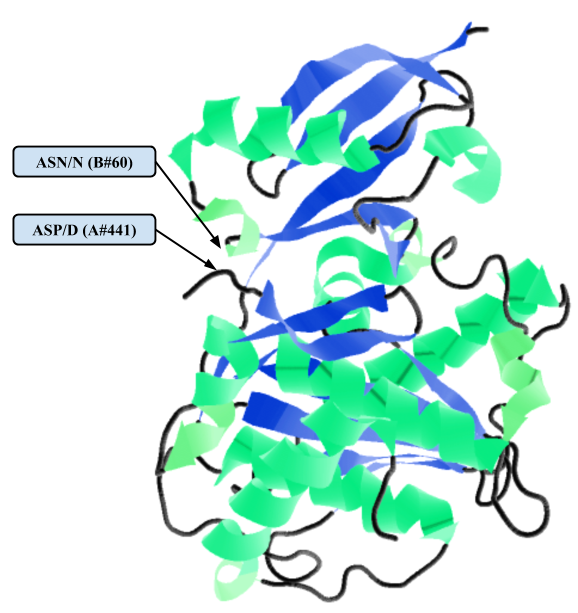
\includegraphics[width=14cm]{figs/gwas_figure_4_jmol.png}
  %\caption{A subfigure}
  \label{fig:sub1}
\end{subfigure}%
\begin{subfigure}{.1\textwidth}
  \centering
  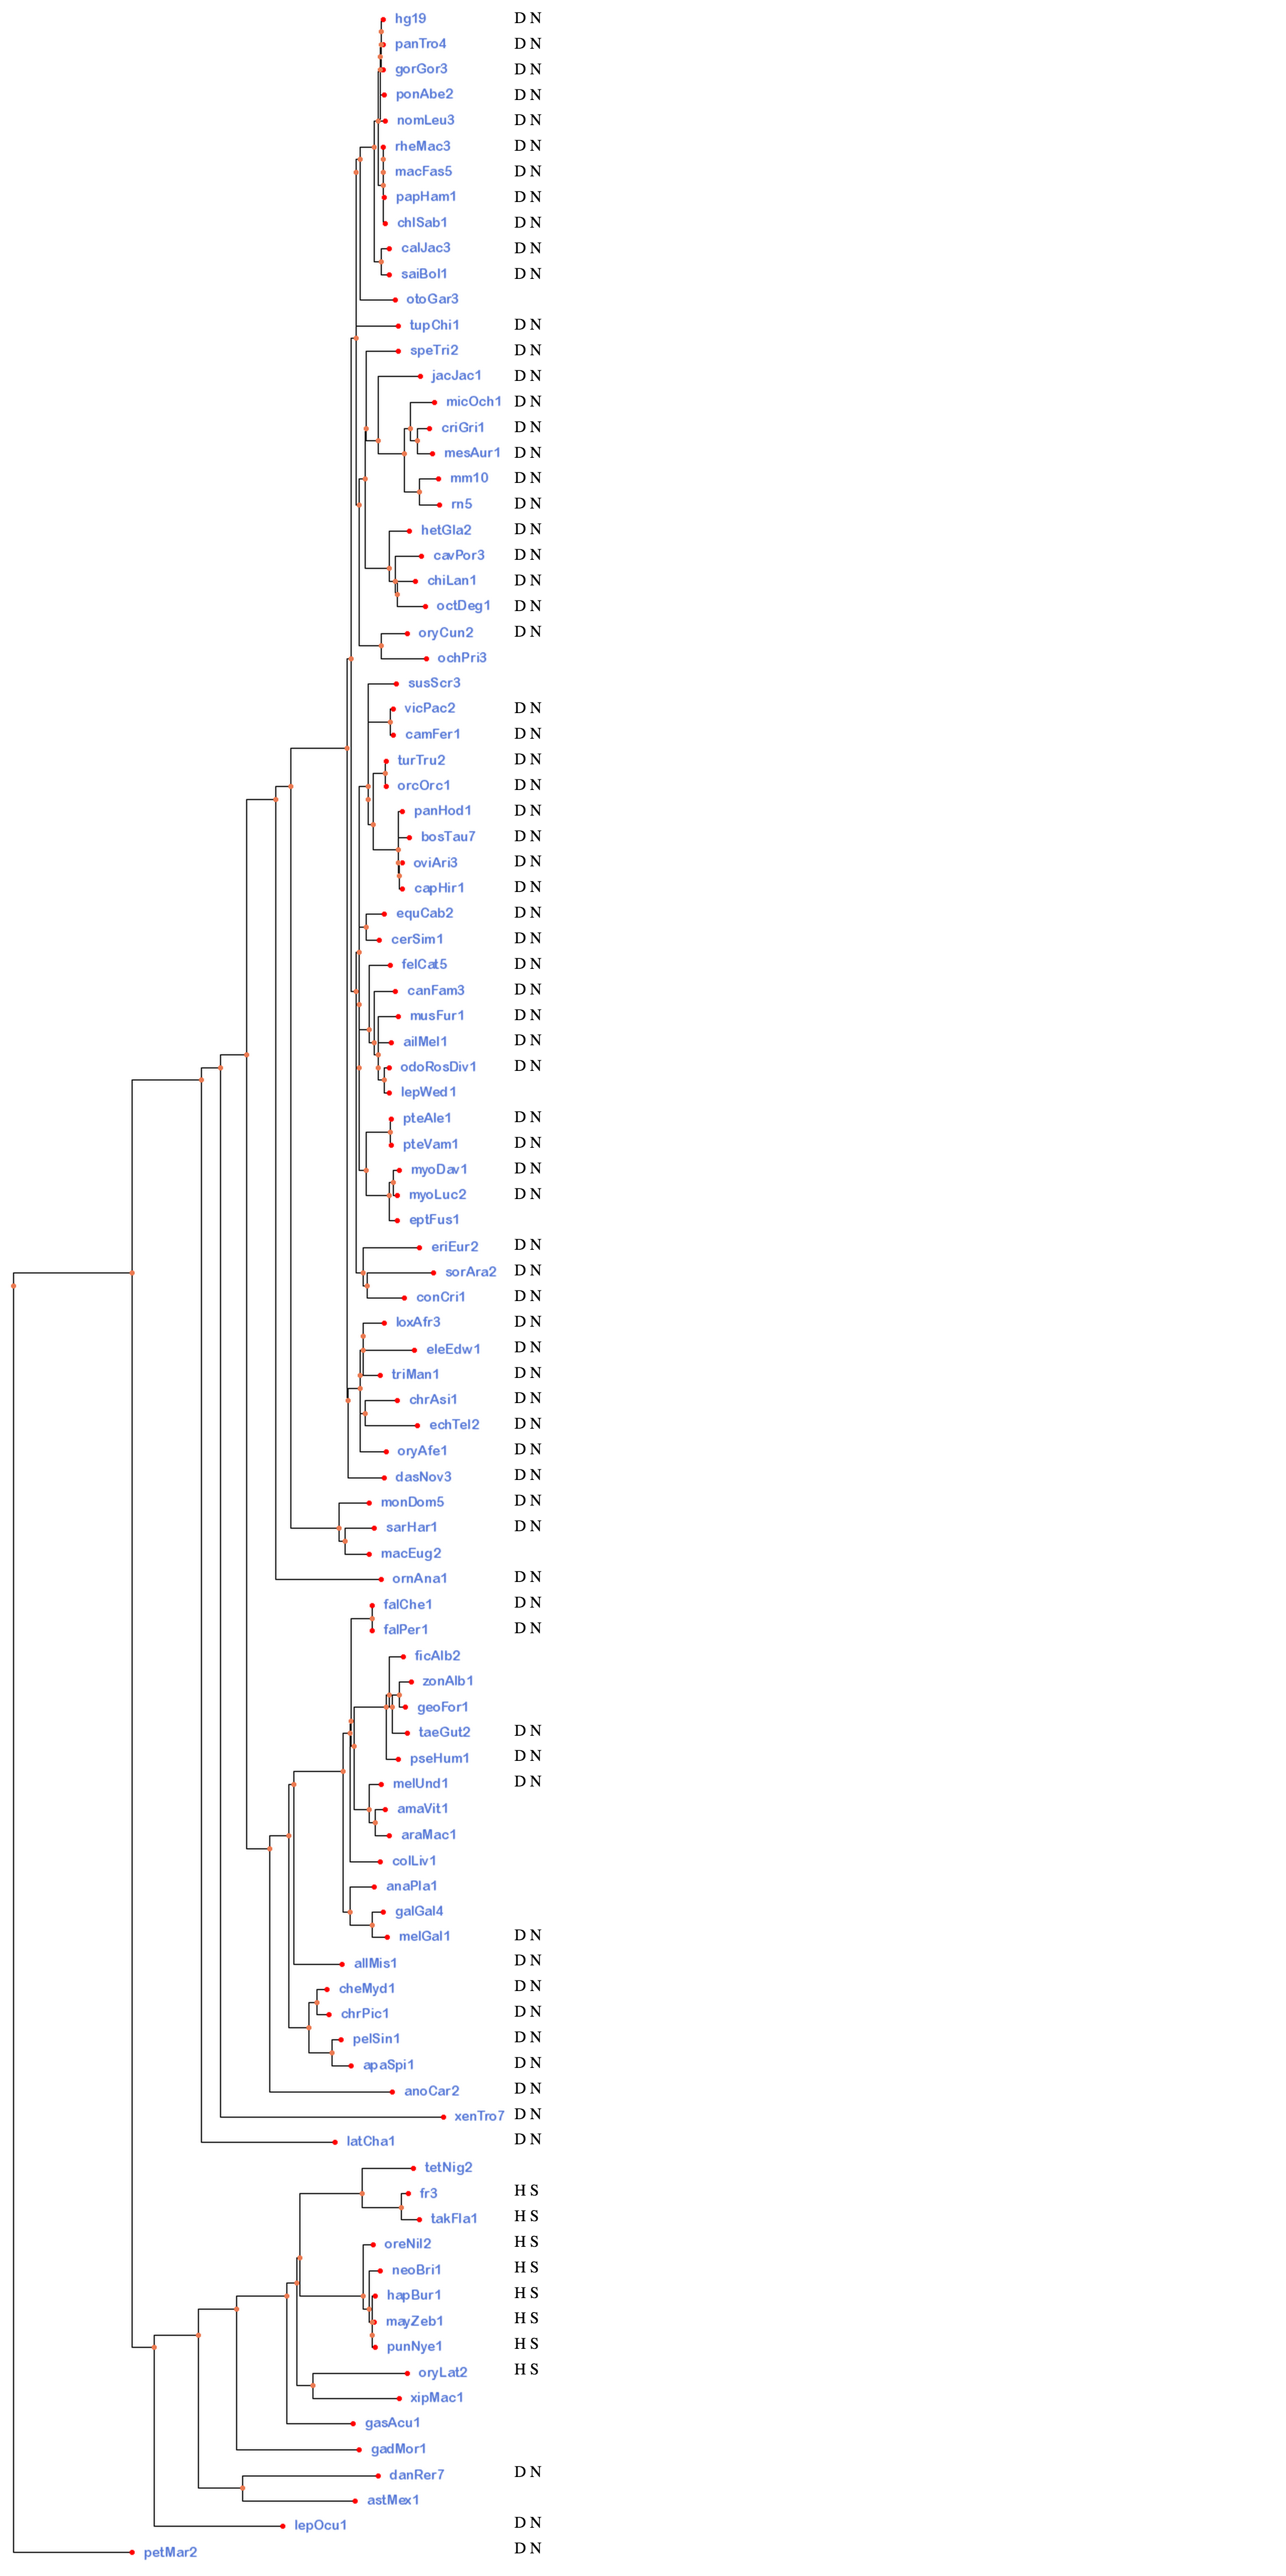
\includegraphics[width=7cm]{figs/gwas_figure_4_tree_coevolution.png}
  %\caption{A subfigure}
  \label{fig:sub2}
\end{subfigure}
\caption{Example of interaction between amino acid \#441 of \textit{Senp1} and \#60 of \textit{Sumo1} proteins detected by our method with $\ell_C = 7.7$. Left: PDB structure 2G4D, shows that the amino acids are in close proximity. Right: Multiple sequence alignment and phylogenetic tree showing the putative compensatory amino acid substitution pair \texttt{D.N} replaced by \texttt{H.S}.}
\label{fig:test}
\end{figure}

Let the two proteins considered have amino acid sequences $A = a_1...a_m$ and $B = b_1...b_n$. To obtain the prediction score for this pair of proteins, we identify the pair of length-$k$ substrings $a_i, a_{i+1}, …, a_{i+k-1}$ and $b_j, b_{j+1}, …, b_{j+k-1}$ that exhibit the strongest support for parallel or anti-parallel interactions

\[
\max\left[ \sum_{l=0}^{k-1}{ \ell_C[ MSA(a_{i+l}) , MSA(b_{j+l}) ]},  \sum_{l=0}^{k-1}{\ell_C[ MSA(a_{i+l}) , MSA(b_{j+k-1-l})} \right]
\]

\noindent where $k=3$ was determined empirically to provide the best predictive power. 
%We calculate the average likelihood ratio of three consecutive pairs of amino acids ($avg_3[LL(M_{SA})]$), either in the forward or reverse directions. For a given pair of genes, we calculate the highest $avg_3[LL(M_{SA})]$ and pick the highest number as representative for that pair. 
As shown in Figure \ref{S5}), prediction accuracy is quite good (p-value $< 2 \cdot 10^{-42}$), considering the modest amount of information considered.

\subsection{Epistatic GWAS analysis}

We applied our methods to a cohort of $\sim 13,000$ individuals in a case-control study of type II diabetes \cite{mccarthy2015T2D}.
This multi-ethnic study covers exons of unrelated individuals from five major ancestral groups (European descent, South Asian, East Asian, Hispanic and African American descent) using an average sequencing coverage over $80 \times$, yielding $1.7$ million coding variants. The filters described in Methods section resulted in a number of variant pairs being analyzed less than $50$ million. By means of the z-score relationship between Bayes Factor and p-values shown in \cite{goodman1999toward}, we can set the GWAS significance threshold for $50$ million pairs at $log_{10}[BF_T] =  8.0$.

\paragraph{Results} Variant annotated and filtered according to the previous paragraphs lead to $\sim 50$ million pairs of variants having high log likelihood in our logistic regression model  ($\ell_G > 6$, in equation \ref{eq:gwasLogLikLogReg}) that were further analysed under co-evolutionary and Bayesian models. The complete analysis took less than $2$ days using a $1,000$ CPU-cluster, thus showing that an epistatic GWAS analysis is feasible using current computational resources. Table \ref{tab:gwas_13k_results_1} shows the main results from our GWAS epistatic analysis, genes highlighted in red belong to a hand curated set of genes either associated with diabetes or known to be in diabetes related pathway. It should be noted that some of the top results include amino acid modification sites such as Phosphoserine (or Glycosylation, not shown), which are likely to b interaction loci.

\figtab{gwas_13k_results_1}{gwas_13k_results_1}{14cm}{Results from epistatic GWAS analysis of type II diabetes sequencing data. First column shows total $log_{10}(BF_T)$; second and third columns show p-value and (raw) Bayes factor for logistic regression model. For each variant in the putative interaction pair: genomic coordinate, gene and functional annotation are shown. Genes marked in red are manually curated gene sets form diabetes related pathways}{Results from epistatic GWAS analysis of type II diabetes sequencing data}

%---
\section{Discussion}
%---

In this paper, we propose a novel methodology for genome wide association studies of pairs of variants under putative epistatic interaction. Due to the large number of statistical tests required in epistatic analysis, and the corresponding reduction of statistical power, this type of analysis is meant to be applied to datasets consisting of large number of samples, but our highly optimized algorithms are suitable for large scale sequencing genomic studies.

We show the application of our methods to a large scale exome sequencing study for type II diabetes consisting of $\sim 13,000$ samples and $\sim 1,7M$ variants. First, this shows the feasible to apply our methods GWAS-scale datasets. 
Second, although larger cohorts are needed in order to find risk alleles that have lower frequencies and are not captured by this study, we show several suggestive association of pairs of putatively interacting variants with type II diabetes. 

The co-evolutionary model we propose in section \ref{sec:gwasQ2} requires multiple sequence alignment and the corresponding phylogenetic tree.
Intuitively, using an $MSA$ with larger number of sequences should improve co-evolutionary model detection and other co-evolutionary approaches indeed require very large $MSA$. But not only such $MSA$ are available only for a small fraction of human proteins, also mixing ortholog and paralog sequences may lead to reduced power. 
Furthermore, both the tree and the number of sequences in the $MSA$ should remain constant throughout the genome in order to take advantage of computational optimizations (matrix exponential precalculation and ``constant tree caching") that allow the algorithm to be applied at genome-wide scale. Some multiple sequence alignments (such as Pfam) usually have different number of sequences for each protein (thus different phylogenetic trees). This poses two main disadvantages for our methodology: i) we cannot benefit from the previously mentioned optimizations, since they require a constant phylogenetic tree throughout the whole genome; and ii) we would add the problem of reconciling different phylogenetic trees from two proteins, which may lead to inconsistencies. 
For all these reasons we selected UCSC's multi-100way \cite{karolchik2014ucsc}, a genome wide multiple sequence alignment of 100 organisms which has single genome wide phylogenetic tree. This $MSA$ is expected to grow with the advent of projects like G10K \cite{haussler2009genome}. 

In order to further validate our co-evolutionary model in the context of human disease, we tested whether it can separate clinically relevant variants from ClinVar database \cite{landrum2013clinvar} according to their clinical significance attribute (CLNSIG). Interestingly, variants categorized as ``benign" or ``druggable" have higher scores (mean $\ell_C$ within protein) than variants categorized as pathogenic (Supplementary Tables \ref{tab:S4A}, \ref{tab:S4B} and Figure \ref{fig:S4}). We speculate that this might be because amino acids that can be compensated would be characterized as ``benign" whereas deleterious amino acids changes cannot be compensated by mutation. 

As future work, we plan to extend our method to include context specific information by creating $Q_2$ estimates for different protein domains. This would allow to obtain better estimates for well characterized protein interaction regions. Another line of work is to perform GWAS using kernel based statistics of multiple variants \cite{wu2011rare} thus allowing simultaneous analysis of nearby variants in a putative interaction hotspot. In this case the epistatic information would be used as a function modifying the kernel, instead of a bayesian prior.
